\chapter{Methods}

\section{The data}
PLease tell where is the data come from, a little brief of company can be put here.
\section {Puad Hamdani/ 1164084}
\subsection {Teori}
\begin{enumerate}
\item Random Forest
\par
Merupakan classifier yang terdiri dari banyak pohon keputusan dan melakukan klasifikasi berdasarkan keluaran dari hasil klasifikasi setiap pohon keputusan anggota
\begin{figure}[ht]
\centering
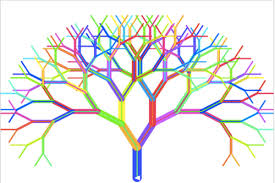
\includegraphics[scale=0.5]{figures/111.JPG}
\caption{Random Forest}
\end{figure}
\item Cara membaca dataset kasus
\begin{itemize}
\item Buka aplikasi spyder untuk membuka dan membaca kodingan dataset
\item Kemudian buat  variable imgatt untuk memasukkan atribut label
\item Lalu uji coba kodingan untuk mengetahui apa hasil dari dataset tersebut
\item imgatt.head() untuk melihat sebagian data awal
\item .shape untuk melihat jumlah data
\item .pivot untuk merubah atribut menjadi kolom
\par
Dengan menguji coba kodingan yang ada pada spyder untuk membaca data set.
\end{itemize}
\item Cross Validation
\par 
Cross Validation adalah teknik validasi model untuk menilai bagaimana hasil analisis statistik (model) akan digeneralisasi ke kumpulan data independen. terutama digunakan dalam pengaturan di mana tujuannya adalah prediksi, dan orang ingin memperkirakan seberapa akurat model prediksi akan dilakukan dalam praktek
\item Arti 44 persen pada RF, 27 persen pada Decission Tree, dan 29 persen pada SVM.
\begin{itemize}
\item Merupakan akurasi dari sebuah pohon keputusan untuk menunjukkan hasil keputusan dengan klasifikasi dari dataset yang ada.
\end{itemize}
\item Confusion Matrix
\begin{itemize}
\item Import confusion matrix
\item Plot confusion matrix
\item Lalu sesuaikan plotnya
\item Setelah itu plot kembali
\end{itemize}
\item Voting
\par
Voting Merupakan metode untuk menentukan keputusan dalam suatu suatu pemilihan, berdasarkan pendapat per orang, dan keputusan ditentukan berdasarkan pemilih terbanyak

\end{enumerate}
\section{Method 1}
Definition, steps, algoritm or equation of method 1 and how to apply into your data
\section{Method 2}
Definition, steps, algoritm or equation of method 2 and how to apply into your data